
\documentclass[12pt]{article}
\usepackage{sbc-template}
\usepackage{graphicx,url}
\usepackage[brazil]{babel} 
\usepackage[utf8]{inputenc} 
\usepackage{indentfirst}
\usepackage{subfigure}
\usepackage[dvips]{epsfig}
\usepackage[ruled,lined,portuguese]{algorithm2e}
\usepackage{algorithmic} 
\usepackage{amsmath}
\usepackage{setspace}


%\def\baselinestretch{0.935} 
\sloppy
%%%%%%%%%%%%%%%%teste do otto
\title{Uma Infraestrutura Ágil e Efetiva de Virtualização de \\Funções de Rede para a Internet das Coisas
\let\thefootnote\relax\footnote{Este trabalho foi realizado com recursos do CNPq, CAPES, FAPERJ e FAPESP (2015/24514-9, 2015/24485-9 e 2014/50937-1).}}
\author{
Diogo M. F. Mattos\inst{1}, 
Pedro B. Velloso\inst{2} e Otto Carlos M. B. Duarte\inst{2}\vspace{-3mm}}
%%otto
%eu colocaria os nomes por extenso, todos
\address{Mídiacom - Departamento de Engenharia de Telecomunicações\\Universidade Federal Fluminense (UFF)\vspace{-3mm}%\\Niterói, RJ -- Brasil
\nextinstitute Grupo de Teleinformática e Automação\\Universidade Federal do Rio de
Janeiro (UFRJ)%\\Rio de Janeiro, RJ -- Brasil
}


\usepackage{hyperref}
\hypersetup{
pdfpagemode=UseOutlines,
colorlinks=true,
a4paper,
breaklinks=true,
linkcolor=black,
anchorcolor=black,
citecolor=black,
filecolor=magenta,
menucolor=red,
urlcolor=black,
bookmarksopen=true,
bookmarksnumbered,
pdfpagelayout=SinglePage,
pdfpagetransition=Dissolve,
pdftitle={VFC: Uma Infraestrutura de Virtualização de Funções de Rede para a Internet das Coisas}, 
pdfauthor={Diogo Menezes Ferrazani Mattos, 
Pedro Braconnot Velloso e Otto Carlos Muniz Bandeira Duarte}, 
pdfproducer={Grupo de Teleinformática e Automação - UFRJ},
pdfcreator={GTA},
pdfkeywords={Rede Virtual, OpenFlow, VirtualBox, Virtual Network, Virtualization,
Virtualização, Router, Roteador, Virtual Router, Roteador Virtual,
Isolamento, Isolation, Flexibility, Flexibilidade, Hibrid, Híbrido} }

\begin{document} 

\maketitle

\begin{resumo} 
%As tecnologias de Internet das Coisas para sensoriamento, monitoramento e governança de cidades aumentam o número de objetos conectados e a criticidade dos dados trafegados. 
As restrições computacionais e de consumo de energia de objetos 
conectados à Internet das Coisas
não os permitem oferecer serviços de redes mais complexos do que o simples envio de dados. 
Em cidades inteligentes, a impossibilidade de prover serviços de segurança e qualidade de serviço pode resultar, até mesmo, 
em desastres nos centros urbanos.
Este artigo propõe a integração vertical de um serviço complexo 
de rede
%de segurança e qualidade de serviços 
em uma nuvem através de uma infraestrutura de virtualização de funções de rede, ágil e efetiva, que provê domínios isolados de objetos conectados. A proposta desenvolve um nó de acesso 
%(\textit{gateway}) 
que virtualiza os domínios em que os objetos se conectam à infraestrutura. 
Um protótipo de serviços de segurança e de qualidade de serviço foi implementado. A avaliação mostra que a virtualização não impacta no desempenho das funções virtuais de rede. A proposta provê segurança aos objetos, identificando tráfego malicioso com acurácia de 99,8\%, evitando a negação de serviços essenciais, e garante a qualidade de serviço.



%O número de objetos conectados enviando dados para serem processados remotamente é crescente. 
%Com a adoção de tecnologias da informação para o monitoramento e governança das cidades, o número de objetos conectados à Internet aumenta e, também, aumenta a criticidade dos dados trafegados. Uma falha na comunicação de um desses objetos com a Internet pode resultar em acidentes ou, até mesmo, desastres em grandes centros urbanos. Este artigo propõe uma infraestrutura de virtualização de funções de rede para Internet das Coisas para implantação ágil e efetiva de domínios isolados de objetos conectados. Cada domínio possui requisitos de desempenho e segurança garantidos por um conjunto funções que executa em uma rede de transporte dotada de recursos de computação em nuvem. Para tanto, a proposta desenvolve um nó de acesso que virtualiza os domínios em que os objetos se conectam. Um protótipo foi implementado e a sua avaliação mostra que a virtualização do acesso não impacta no desempenho das funções virtuais de rede. Os resultados mostram ainda que a proposta provê segurança aos objetos conectados, identificando tráfego malicioso com uma acurácia de 99,8\% e garante qualidade de serviço ao tráfego legítimo, evitando a negação de serviços essenciais. 

\end{resumo}

\begin{abstract}

%%% Pedro:
Devices of Internet of Things suffer from severe processing and power constraints, which hinders offering complex network services, other than simple data transmission. In smart city scenarios, the lack of these services, such as security and quality of service, might lead to low performance that can result in disasters in urban centers.
%The processing and power-consumption constraints of the Internet of Things devices do not allow them to offer more complex network services than the simple data transmission in smart city scenarios.
%The lack of such services, such as security and quality of service, can even result in disasters in urban centers.
%%% Pedro: aqui não entendi nada. Não consegui nem sugerir mudanças   :(
%Diogo: Dei uma mudada... Vê o que vc acha
In this paper, we propose an agile and effective network function virtualization infrastructure of isolated domains of connected devices, which outsources network tasks from the devices to the networking cloud.
%%% Pedro:
The domain isolation is achieved by virtualizing the gateway access node to which IoT devices connect.
%To do so, our proposal develops a gateway access node that virtualizes the domains in which the devices connect. 
%%% Pedro:
We have deployed a prototype to provide security and quality of service to IoT applications. Preliminary results show that the gateway virtualization does not impact the performance of virtual network functions.
%A prototype for services of security  and quality of service has been implemented and its evaluation shows that virtualization of the access node does not impact the performance of virtual network functions. 
%%% Pedro:
Additionally, our proposal provides security for connected devices, identifying the mallicious traffic with 99.8\% accuracy, avoiding denial of essential services, and ensuring quality of service.
%The results also show that the proposal provides security for connected devices, identifying the traffic of threats with 99.8\% accuracy, avoiding denial of essential services, and ensuring quality of service.

\end{abstract}


%1,5 página - Introdução

\section{Introdução}
\label{sec:introducao}
%%% Otto
%%%%Otto
%%%%Adorei :) Nada a acrescentar
%%motivação de cidades inteligente bem feita
%%Tirei da ONU --> https://esa.un.org/unpd/wup/Publications/Files/WUP2014-Report.pdf
Em um mundo cada vez mais interconectado, estima-se que atualmente 54\% da população viva em cidades e que esse número alcance 66\% em 2050 \cite{relatorio-onu}. 
%O crescimento previsto previsto para o número de pessoas vivendo em cidades deve concentrar-ser na África e na Ásia. 
%No mundo cada vez mais global e interconectado de hoje, mais de metade da população mundial (54\%) vive agora em áreas urbanas, ante 30\% em 1950. As próximas décadas trarão mudanças profundas no tamanho e na distribuição espacial do mundo população de modo que a população mundial em 2050 seja projetada para ser 66\% urbana. Prevê-se que a população urbana global cresça 2,5 bilhões de habitantes urbanos entre 2014 e 2050, com quase 90\% do aumento concentrado na Ásia e na África. 
Para responder a desafios decorrentes do crescimento acelerado das cidades e alavancar as oportunidades geradas pela urbanização contínua, as políticas governamentais devem convergir esforços para focar na sustentabilidade das áreas urbanas. Uma alternativa para garantir a sustentabilidade é implantar e expandir os serviços públicos inteligentes, a distribuição de energia e água inteligentes, os serviços de saúde inteligentes e a governança das cidades baseada em plataformas de coleta de dados e tomada de decisões~\cite{petrolo,interscity-paper}. %Dessa forma, a adoção de plataformas de cidades inteligentes é essencial para a urbanização sustentável.

O desenvolvimento de plataformas para cidades inteligentes está associado ao 
sensoriamento, monitoramento e atuação sobre diversos objetos conectados no contexto urbano~\cite{zhang-security} que, por sua vez, são uma aplicação do conceito de Internet das Coisas (\textit{Internet of Things} - IoT)~\cite{petrolo}. 
No entanto, a conexão dos objetos depende de dispositivos de comunicação que estão sujeitos a severas restrições de processamento e consumo de energia. Tais restrições impossibilitam o provimento de serviços de redes mais complexos como segurança e qualidade de serviço, sem os quais, grande parte das aplicações de cidades inteligentes têm o desempenho prejudicado ou até mesmo inviabilizado. Portanto, o objetivo principal deste trabalho é prover serviços complexos de redes 
para aplicações de IoT, %sem acrescentar sobrecarga à rede. 
%O objetivo é alcançado pela 
através da terceirização das funções de redes para uma infraestrutura virtualizada na nuvem.
%Este objetivo é alcançado através da virtualização dos pontos de acesso da rede IoT e da utilização de funções de redes virtualizadas em nuvem.

%%% Pedro: eu cortaria o trecho abaixo, caso coloque a sugestão acima.
%Assim, a interconexão de objetos no contexto urbano vai além de simplesmente criar domínios de rede de sensores desconexos ou com padrões distintos. No contexto de cidades inteligentes é necessário criar uma infraestrutura ágil de rede de transporte para Internet das Coisas que seja capaz de assumir tarefas de rede especializadas ante a execução dessas tarefas em sensores ou objetos com pequeno poder computacional. %Contudo, as principais abordagens para plataformas de cidades inteligentes focam em qual tecnologia usar no enlace de comunicação com os sensores~\cite{lorawan}, na captura e no tratamento dos dados~\cite{petrolo,interscity-paper} ou na gerência da rede de IoT~\cite{sdn-iot,globecomm-nfv-iot}.

Este artigo propõe reduzir a carga do processamento dos objetos conectados através uma infraestrutura de virtualização de funções de rede para Internet das Coisas. A ideia principal é que cada domínio de IoT seja uma fatia vertical da rede de transporte que comporta desde o nó de acesso até a interface com o consumidor dos dados. Para tanto, a proposta desenvolve um nó de acesso sem-fio, chamado de \textit{gateway}, que multiplexa o acesso à rede através de criação de pontos de acesso virtuais e conecta os objetos da rede sem-fio a uma infraestrutura de virtualização de funções de rede (\textit{Network Function Virtualization Infrastructure} - NFVI). Na NFVI, são executadas funções virtuais de rede (\textit{Virtual Network Function} - VNF) que assumem o processamento dos pacotes ao invés de deixá-lo para os objetos conectados ou para o \textit{gateway}. %Este artigo propõe ainda uma VNF de classificação de tráfego capaz de identificar tráfego malicioso em um domínio IoT com acurácia de 99,8\% e, também, uma outra VNF capaz de conformar o tráfego dos objetos conectados e evitar a negação de serviços essenciais.

Trabalhos anteriores focam em plataformas de coleta e tratamento de dados~\cite{petrolo,zhang-security,interscity-paper} ou em modelos teóricos de como gerenciar as redes de IoT~\cite{sdn-iot,sdn-nfv-iot,globecomm-nfv-iot}. A proposta deste artigo é a virtualização do nó de acesso dos domínios de IoT combinado com uma infraestrutura de virtualização de funções de rede ágil e efetiva na implantação das funções. A infraestrutura de virtualização é capaz de assumir funções de tratamento de pacotes, antes desempenhadas por objetos conectados, e, assim, realiza a classificação de tráfego e a reação a ataques implementadas como funções virtuais. Um protótipo da proposta foi implementado e a sua avaliação mostra que o atraso na comunicação entre o nó de acesso e a infraestrutura não é significativo  e que a virtualização do ponto de acesso não impacta no desempenho das funções virtuais de rede. Os resultados mostram ainda que a VNF de classificação identifica o tráfego malicioso em um domínio IoT com acurácia de 99,8\% e, também, outra VNF provê qualidade de serviço para os objetos conectados e evita a negação de serviços essenciais.%, limitando o tráfego de ataque.
%Ademais, verifica-se também que a classificação de tráfego é efetiva e que a infraestrutura é capaz de isolar ataques de negação de serviço no domínio IoT sem afetar os serviços críticos.

O restante do artigo está organizado da seguinte forma. O serviço de rede para a Internet das Coisas é detalhado na Seção~\ref{sec:net-iot}. Na Seção~\ref{sec:infra}, propõe-se a infraestrutura de virtualização de funções para Internet das Coisas. A avaliação da proposta discutida na Seção~\ref{sec:results}. A Seção~\ref{sec:relacionados} discute os trabalhos relacionados. A Seção~\ref{sec:conclusao} conclui o artigo.


\section{O Serviço de Rede para Internet das Coisas}
\label{sec:net-iot}


\begin{figure}[t!]
\begin{center}
\mbox{
\subfigure[Esquema de uma plataforma para Internet das Coisas.]{
\label{fig:iot-arch:a}
\includegraphics[width=0.45\textwidth]{figs/iot-fisico-virtual.png}}
}
\hspace{1mm}
\mbox{
\subfigure[Arquitetura de uma plataforma para cidades inteligentes.] {
\label{fig:topos:b}
\includegraphics[width=0.45\textwidth]{figs/smart-city.png}}
}
\end{center}
\vspace{-3mm}
\caption{Arquitetura de referência para implantação de cidades inteligentes. (a) Esquema do relacionamento entre dispositivos físicos e aplicações virtuais para prover serviços de Internet das Coisas. (b) Arquitetura de exemplo de cidade inteligente, em que a comunicação entre sensores e aplicações é intermediada interfaces de acesso à rede, processamento e armazenamento. A plataforma de cidades inteligentes age como um \textit{middleware}.}
\label{fig:topos}
\vspace{-4mm}
\end{figure}

%As principais tecnologias habilitadoras para Internet das Coisas são comumente definidas em quatro camadas princiapis: dispositivos físicos de identificação e sensoriamente, \textit{middleware}, aplicações virtuais e composição de serviços e infraestrutura virtual de nuvens para abstração de objetos~\cite{survey-morabrito}. 
A arquitetura de referência para Internet das Coisas, Figura~\ref{fig:iot-arch:a} evidencia a transição entre os dispositivos físicos e as abstrações em \textit{software} para aplicações de IoT. 
%livro de IoT
Nesse sentido, o desenvolvimento de sensores, etiquetas de identificação e tecnologias de comunicação entre sensores são agrupadas na categoria de comunicação entre objetos.  A interação entre as aplicações e os objetos no mundo real são intermediadas por um \textit{middleware}, um \textit{software} de adaptação de requisições para cada tipo de objeto~\cite{interscity-paper}. A ideia básica do \textit{middleware} é abstrair os objetos em microsserviços e prover serviços mais complexos através da composição dos microsserviços simples. 
%A adoção dos princípios de arquitetura orientada a serviços (SOA) permite a decomposição de sistemas complexos e monolíticos em aplicações que consistem em um ecossistema de componentes mais simples e bem definidos~\cite{survey-morabrito}.
As aplicações, por sua vez, usam os serviços providos e gerenciados pelo \textit{middleware} para sensoriar dados ou atuar em diferentes contextos. 
%Paralelamente, a computação em nuvem é apontada como uma tecnologia habilitadora da Internet das Coisas, já que permite o processamento em tempo hábil dos diversos dados capturados pelos objetos conectados e enviados ao \textit{middleware}. 
Contudo, nessa visão, oculta-se as especificidades do serviço de rede necessárias para cada tipo de aplicação. Assim, aplicações em tempo real, como as industriais~\cite{industria4.0}, usam o mesmo serviço da rede de transporte que aplicações com requisitos menos estritos de latência, mas sensíveis à privacidade dos dados.

%bluetooth, zigbee, wifi, celular, zigfox, lorawan
%IP6LowPAN
Considerando as redes de acesso, é possível definir redes de curto, médio e longo alcance para atender os objetos conectados. Entre os meios de acesso de curto alcance destacam-se as tecnologias baseadas em Bluetooth Low Energy (BLE) e Zigbee que apresentam como principais características o uso da frequência base de 2.4~GHz e o baixo consumo de energia. Comparando o BLE e o Zigbee, o BLE é mais eficiente em termos energéticos, já que o consumo de energia por bit transmitido é menor~\cite{iot-protocols}, o que implica maior custo de {\it hardware} do BLE. Em redes de médio alcance, destaca-se o uso do WiFi (IEEE~802.11) como protocolo de acesso~\cite{wifi-iot}, devido a popularização de equipamentos compatíveis e a facilidade de desenvolvimento de aplicações. Ao se considerar redes de longo alcance, em grandes cidades é comum o uso de redes de celulares 3G/4G para o sensoriamento e aquisição de dados. Essa alternativa apresenta alta taxa de transmissão, mas implica grande gasto energético dos dispositivos e necessidade de cobertura de rede de celular. Em áreas com pouca infraestrutura e para aplicações que não requerem altas taxas de transmissão, os protocolos LoraWAN~\cite{lorawan} e ZigFox\footnote{http://makers.sigfox.com/.} são alternativas ao uso de redes de celulares para conectar objetos. Ambas tecnologias usam bandas estreitas para cobrir grandes áreas de alcance, com baixo consumo de energia e, consequentemente, baixa taxa de bits transmitidos. Vale ressaltar ainda o uso do protocolo 6LowPAN~\cite{6lowpan} como protocolo de rede para baixo consumo de energia. O protocolo de rede 6LowPAN define encapsulamento e mecanismos de compressão de cabeçalho. O padrão suporta diversas tecnologias de acesso, como Ethernet, IEEE~802.11 e IEEE~802.15.4.
%
Na camada de aplicação, o protocolo para serviços Web na Internet das Coisas, definido pelo IETF, é o Protocolo de Aplicação Restrita ({\it Constrained Application Protocol} - CoAP). O CoAP é um protocolo de transferência de dados sem estados que inclui um subconjunto de funcionalidades do HTTP. O CoAP foi re-projetado para operar com baixo poder de processamento e com restrição de gasto de energia em objetos conectados para comunicação entre dispositivos ({\it Machine to Machine} - M2M)~\cite{iot-miguel,coap}.
%De forma semelhante ao HTTP, o CoAP identifica recursos usando um identificador universal de recurso ({\it Universal Resource Identifier} - URI) e define métodos para acesso e modificação do recurso, como GET, PUT, POST e DELETE. A principal diferença entre o CoAP e o HTTP é que o primeiro é um protocolo de transporte por si só, enquanto o HTTP usa o TCP para realizar o transporte. Em cenários de vários dispositivos com fluxos de pouca duração e com possibilidade de erros no meio, o TCP gera grandes sobrecargas de retransmissão, processamento e latência, enquanto o CoAP foi projetado para manter o tamanho da mensagem mínimo, evitando fragmentação e com a possibilidade de envio mensagens com confirmação ou sem confirmação~\cite{coap}.

As tecnologias habilitadoras da Internet das Coisas aplicadas ao sensoriamento e à governança de cidades caracterizam as cidades inteligentes~\cite{interscity-paper}. 
A Figura~\ref{fig:topos:b} resume uma infraestrutura de referência para cidades inteligentes. No contexto de cidades inteligentes, o serviço de rede passa a ter um papel fundamental no transporte dos dados dos objetos até a plataforma de processamento e armazenamento de dados. 
%%% Pedro:
Estas plataformas, mostradas na Figura~\ref{fig:topos:b}, normalmente
%As plataformas de processamento e armazenamento de dados mostradas na Figura~\ref{fig:topos:b} normalmente
%%% Cortaria a frase acima.
são realizadas através da computação em nuvem e fornecem interfaces entre as aplicações de gerenciamento e governança da cidade e os dados coletados. Paralelamente, aplicações de gerenciamento e controle em tempo real, como ferramentas de mercado, gerenciamento de operações e gestão de segurança, devem operar sobre dados sensoreados com latência mínima e, assim, devem ter acesso direto aos dados.
%Dessa forma, o serviço de rede de transporte para cidades inteligentes deve ser consciente de quais são os consumidores dos dados e prover serviços diferenciados. 
Vale ainda ressaltar que a infraestrutura de rede de transporte passa a ser responsável pela adaptação entre diferentes protocolos de comunicação entre objetos, assim como por filtrar e agregar os dados monitorados. % para cada aplicação.
%%% Pedro: esta adapatação dos dados (acima) ficou meio solta. O que é a adaptação dos dados?
%Diogo: dei uma melhorada. Veja se gosta assim.


%Comparação
%A proposta deste artigo complementa as plataformas para Internet das Coisas atuais e propõe um serviço da rede de transporte adptado para as aplicações de Internet das Coisas, através de um \textit{gateway} de acesso para os objetos conectados a uma nuvem de virtualização de funções de rede. O tráfego proveniente dos objetos conectados é classficado e encadeado em cadeias de funções específica para cada aplicação. Com isso, tanto os objetos como o \textit{gateway} de acesso têm recursos computacionais liberados, já que o processamento dos pacotes na rede, o roteamento, a conformação de políticas e o enfileiramento passam a desempenhados pela nuvem. É importante que o serviço de rede seja capaz de abstrair a tecnologia de acesso usada pelos objetos conectados e consiga adaptar dados entre protocolos de aplicação dedicados a IoT, como o CoAP, e protocolos de aplicação de uso geral, como o HTTP.


\section{A Infraestrutura Proposta}
\label{sec:infra}

%%% Pedro: aqui foi que conversamos e que não concordo tanto. Para mim, os requisitos são os mesmos das redes "convencionais". A diferença é que os dispositivos que formam a rede não têm capacidade de prover serviços de rede que garantam estes requisitos. 
%%% Aí entra a sua proposta.
%%% Lembre que eu focaria também no fato que você está também "aliviando" o ponto de acesso da sobrecarga que usualmente outros trabalhos impõe, tentando prover alguns dos serviços de rede. Assim, o ponto de acesso poderia atender um número maior de redes e por consequência, um número maior de aplicações. 
%%% O que achou?
%Diogo: Adicionei uma frase sobre terceirização do processamento na introdução. Vou tentar deixar isso claro.
%%% Se achou que o que falei é válido, acho que poderia ter uma menção na intro, como vantagem. Não coloquei nas minhas sugestões da intro, pois fiquei na dúvida se isso é um fato realmente da sua abordagem.
Os requisitos de rede dos objetos conectados em um cenário de Internet das Coisas são mais críticos do que redes convencionais em função da integração vertical das aplicações, chamados de silos, e da magnitude da comunicação entre dispositivos ({\it Machine to Machine} - M2M)~\cite{how-sdn-nfv-iot}. Segurança, mobilidade, escalabilidade, adequação a políticas e qualidade de serviço são requisitos essenciais e  
% Diogo: Adicionei o trecho:
críticos de serem providos por objetos com restrições de processamento e gasto de energia.
%
%o que achou?
Nesse sentido, a infraestrutura proposta age de forma a prover um serviço de rede baseado no encadeamento de funções~\cite{sbseg-nfv} capaz de executar funções virtuais de rede (\textit{Virtual Network Function} - VNF) terceirizadas pelos objetos conectados. 
%%% Pedro: na frase a baixo, ficou estranho dizer que introduz a ideia do gateway, pois em geral, as aplicações de IoT já consideram a existência de um gateway. Não seria melhor dizer que introduz a ideia de um gateway virtualizado no equipamento que serve como ponto de acesso. Ou algo do tipo.
%ok
Para tanto, a proposta introduz a ideia de um {\it gateway} virtualizado no equipamento de acesso dos objetos conectados ao ambiente de virtualização de rede, mostrado na Figura~\ref{fig:arch}. Ao conectar os objetos à infraestrutura de virtualização de redes, o {\it gateway} executa somente o encaminhamento dos quadros que chegam a ele pelas interfaces virtuais de rede e todo processamento dos pacotes, adaptação de protocolos, conformação de políticas, qualidade de serviço ou análise de conteúdo, é realizado pela infraestrutura de virtualização de redes através de funções virtuais de rede.

\begin{figure}
\begin{center}
 \includegraphics[width=0.99\textwidth]{figs/arquitetura-iot-nfv.png}
 \end{center}
\vspace{-3mm}
\caption{A infraestrutura de virtualização de funções de rede para Internet das Coisas. O \textit{Gateway} de Objetos Conectados abstrai o método de acesso através de interfaces virtuais conectadas por túnel à Infraestrutura de Virtualização de Funções de Rede (NFVI). O \textit{gateway} envia os quadros direto para a NFVI. %O processamento dos dados na camada de rede e superiores é realizado pela NFVI.
} 
\label{fig:arch}
\vspace{-3mm}
\end{figure}

\subsection{O \textit{Gateway} de Acesso}

A ideia principal do \textit{gateway} é criar interfaces virtuais que ajam como diferentes pontos de acesso virtuais para diferentes domínios de objetos conectados. O {\it gateway} é realizado sobre um {\it hardware} que possui recursos físicos para implantar interfaces virtuais de rede, seja uma interface sem-fio IEEE~802.11, IEEE~802.15.4, uma estação base LTE ou outras tecnologias. Por simplicidade, neste trabalho considera-se um {\it gateway} equipado com uma placa de rede sem-fio IEEE~802.11n. Dessa forma, os objetos se conectam às redes cujo acesso é provido pelo {\it gateway}. No entanto, a função do {\it gateway} resume-se a prover a realização física do ponto de acesso, o que está alinhado com as propostas de redes 5G e C-RAN ({\it Cloud Radio Access Network})~\cite{cran}. Após a conexão, todos os quadros são encaminhados para infraestrutura de virtualização de redes através de um túnel GRE\footnote{Acessível em https://tools.ietf.org/html/rfc2784.} (\textit{Generic Routing Encapsulation}). Vale ressaltar que a conexão entre o {\it gateway} e a infraestrutura de virtualização de redes pode ocorrer através da Internet e, portanto, está sujeita a atrasos e perda de pacotes. 

A virtualização das interfaces de rede sem-fio é realizada através da criação de um ponto de acesso virtual no \textit{gateway}, usando a aplicação \texttt{hostapd}\footnote{Disponível em https://w1.fi/hostapd/.} em consonância com os utilitários \texttt{iw-utils}\footnote{Disponível em http://drvbp1.linux-foundation.org/~mcgrof/rel-html/iw/.}. Dessa forma, a configuração dos pontos de acesso virtuais permite que um mesmo \textit{gateway} forneça serviço de conectividade a diferentes domínios de IoT, garantindo assim o isolamento na camada física já que cada ponto de acesso virtual pode possuir suas próprias credenciais de autenticação e acesso. Com credenciais de acesso distintas, o participante de um domínio de IoT não é capaz de bisbilhotar os demais domínios virtuais, já que a criptografia na camada física é diferente para cada ponto de acesso virtual.


\subsection{A Infraestrutura de Virtualização de Redes}

A virtualização de funções de rede ({\it Network Function Virtualization} - NFV) caracteriza-se pela adoção de tecnologias de computação em nuvem, em especial da tecnologia de virtualização, no domínio de redes de transporte, permitindo a virtualização de funções de rede implementadas em {\it software}~\cite{survey-tarik}. A Figura~\ref{fig:arch} mostra a infraestrutura de virtualização de redes baseada na arquitetura de referência de gerência e orquestração de funções virtuais de rede ({\it Network Function Virtualization MANagement and Orchestration} - NFV-MANO)~\cite{etsi-nfv-mano}. Na NFVI, os recursos físicos da rede são abstraídos em recursos virtuais e, nos ambientes virtuais, funções virtuais de rede são implementadas em {\it software} e encadeadas para prover serviços de rede complexos. O comportamento do serviço de rede para cada silo de IoT depende do encadeamento de diferentes VNFs. 

Ao chegar um novo pacote na NFVI, esse pacote é direcionado a uma das cadeias de funções de serviço ({\it Service Function Chain} - SFC) existentes na infraestrutura. Uma cadeia de funções de serviço consiste no sequenciamento de funções virtuais de rede pelas quais o pacote deve seguir. Vale ressaltar que o sequenciamento correto das funções, assim como a escolha adequada das funções na cadeia, definem o comportamento do serviço de rede que o pacote encontra ao atravessar a NFVI. Para direcionar os pacotes para a cadeia de funções de serviço correta, a NFVI emprega um classificador logo após a entrada do pacote. O classificador marca o pacote com a etiqueta correta da SFC responsável por tratar o pacote. 

%Classificação dos pacotes é dividida em duas etapas. A primeira consiste na decisão de qual cadeia de serviço deve tratar os pacotes. Para tanto, desenvolve-se um classificador baseado em aprendizado de máquina que identifica características comuns do pacote e o encaminha em uma determinada cadeia. A segunda etapa consiste na marcação dos pacotes para direcioná-los na cadeia correta. 

A marcação da cadeia de função de serviços pode ser realizada com o protocolo de cabeçalho de serviço de rede ({\it Network Service Header} – NSH)~\cite{sameer-neo-nsh,nsh-ietf-draft-12}. O direcionamento do tráfego para a SFC correta baseia-se em dois campos principais do protocolo, o SPI e o SI. O SPI, {\it Service Path Identifier}, identifica o caminho de serviço que o pacote deve seguir. Nesse contexto, um caminho de serviço é a sequência de funções virtuais que compõem o encadeamento de funções. O campo SI, {\it Service Index}, identifica em qual posição do caminho de serviço o pacote se encontra e, assim, permite identificar qual é a função virtual de rede correta para tratá-lo no momento. Contudo, as implementações disponíveis para o protocolo NSH ainda são iniciais e o desempenho alcançado não é satisfatório~\cite{sbseg-nfv}. Portanto, uma alternativa viável para estabelecer um caminho de serviço coerente e com bom desempenho é o uso de outros protocolos de encapsulamento bem estabelecidos, tais como GRE e VXLAN, para criar o encadeamento de funções de serviço. Neste trabalho, usa-se o protocolo GRE para implementar o encadeamento de funções de serviço.

\subsection{As Funções Virtuais de Rede}

As funções virtuais de rede consistem de ambientes virtuais que executam funções de tratamento de pacotes. Em uma arquitetura tradicional de Internet das Coisas, essas funções são exercidas pelos objetos conectados ou pelo {\it gateway} de acesso da rede de objetos conectados à Internet. Na infraestrutura proposta, tanto os objetos conectados quanto o {\it gateway} não necessitam de recursos para exercer as funções de rede, pois essas são terceirizadas para a NFVI sob a forma de funções virtuais de rede. Neste trabalho, as funções virtuais de rede são implementadas em máquinas virtuais executando Linux Ubuntu 16.04 %\footnote{Disponível em http://www.ubuntu.com/.}
e com suporte ao comutador por {\it software} Open vSwitch\footnote{Disponível em http://docs.openvswitch.org/}.

%%%%%%%%VNF de classificação de tráfego
%%%%%%%%VNF de QoS
Propõem-se ainda duas VNFs dedicadas ao ambiente de IoT. A primeira classifica o tráfego de cada domínio de IoT entre legítimo ou malicioso através de algoritmos de aprendizado de máquina. A segunda aplica políticas de qualidade de serviço ao tráfego através do encaminhamento de fluxos por filas com recursos previamente definidos. O encaminhamento dos fluxos para as filas corretas é executado por regras em um comutador por \textit{software} instanciado como função virtual de rede.

\subsection{O Consumidor dos Dados}

O consumidor dos dados na infraestrutura proposta é qualquer agente que acesse objetos conectados. No caso de uma câmera de vigilância IP, por exemplo, o consumidor de dados pode ser um portal {\it web} que acessa as imagens capturadas pela câmera e encaminhadas e tratadas pela NFVI. Nesse caso, a NFVI enriquece o serviço de rede de transporte fazendo \textit{cache} do fluxo de dados vindo da câmera e também adaptando o fluxo de dados da câmera para o padrão suportado pelos usuários finais ou pelo portal {\it web}. No caso de os objetos conectados serem uma rede de sensores e atuadores, o consumidor dos dados pode ser um {\it middleware} para IoT que se conecta diretamente à NFVI, sem a necessidade de gerenciar e controlar o acesso dos sensores à rede.

A implementação da infraestrutura proposta considera a \textit{Open Platform for Network Function Virtualization} (OPNFV)
%\footnote{Disponível em http://www.opnfv.org/.} 
como infraestrutura de virtualização de rede que é a plataforma de referência da arquitetura de NFV padronizada pela {\it European Telecommunications Standards Institute} (ETSI). A gerência da camada de virtualização é realizada pelo OpenStack.
%\footnote{Disponível em http://www.openstack.org/.}. 
Para classificar, marcar o fluxo de entrada na NFVI e encaminhá-lo para a cadeia de funções corretas, utilizou-se o Open vSwitch.

\section{Resultados Experimentais}
\label{sec:results}

O protótipo da infraestrutura de virtualização de redes para Internet das Coisas proposta foi desenvolvido baseado na plataforma OPNFV. O ambiente instalado sobre a OPNFV conta com quatro nós equipados com processador Intel Core~i7-4770, 3.40~GHz, 32~GB de RAM e placa de rede Intel \textit{gigabit}. A configuração do ambiente é organizada com um nó agindo como controlador de gerenciamento da nuvem OpenStack e controlador de rede definida por \textit{software} OpenDaylight;
%\footnote{Disponível em https://www.opendaylight.org/.}
 os três outros nós são dedicados à virtualização de processamento e memória, através do Linux KVM,
%\footnote{Disponível em http://www.linux-kvm.org/.}
 e ao armazenamento distribuído em disco através do Ceph.
%\footnote{Disponível em http://ceph.com/.}. 
Todas as versões de \textit{software} usados no ambiente são as de referência da distribuição do OPNFV Danube 3.0\footnote{Disponível em https://www.opnfv.org/software/downloads/release-archives/danube-3-0.}. O \textit{gateway} de acesso dos objetos conectados ao ambiente OPNFV foi implementado sobre um computador equipado com processador Intel Core~i7-2600, 16~GB de RAM, uma placa de rede Intel \textit{gigabit}, para acesso à NFVI, e placa de rede sem-fio, IEEE 802.11n, Ralink RT2870 USB, para criação dos pontos de acesso virtuais. Durante a avaliação do protótipo, foram usados como objetos conectados dois computadores portáteis, equipados com processador Intel Core~i5-2410M, 6~GB de RAM e interface de rede sem-fio embutida, e uma câmera IP, sem-fio, D-Link DCS-5020L.

A avaliação da proposta é dividida em quatro etapas. A primeira etapa verifica o desempenho da conexão da rede de objetos à infraestrutura de virtualização de rede em cenários em que há diferentes atrasos na comunicação entre o \textit{gateway} e a NFVI. O atraso adicionado simula a conexão entre \textit{gateway} e NFVI como uma conexão através de uma rede de larga escala (WAN) e é adicionado com uma variação de 10\% através da ferramenta \texttt{tc} (\textit{Traffic Control}\footnote{Documentação em http://lartc.org/manpages/tc.txt.}). A segunda etapa avalia a sobrecarga da virtualização da interface de rede sem-fio. A terceira etapa compara o desempenho de três algoritmos de classificação baseados em aprendizado de máquina para identificar tráfego malicioso e tráfego legítimo na rede de objetos conectados. Por fim, a quarta etapa da avaliação testa a efetividade da infraestrutura de virtualização de rede proposta para proteger a rede de objetos conectados de ataques e prover qualidade de serviço a tráfegos prioritários. Todos os resultados apresentados são médias com intervalo de confiança de 95\%.

Na primeira etapa da avaliação, os experimentos visam aferir a taxa máxima de pacotes enviadas pelos objetos conectados e recebidas por consumidores de dados. Nesse experimento, como objeto conectado foi usado o computador portátil. A Figura~\ref{fig:taxas} compara as taxas máximas obtidas para o envio de 10~mil, 50~mil e 100~mil pacotes/s, para pacotes pequenos de 64~B e pacotes grandes de 1.200~B. Vale ressaltar que na infraestrutura criada a unidade de transferência máxima (MTU) foi configurada para 1.280~B devido às sobrecargas com encapsulamentos. O envio de pacotes foi realizado através da criação de fluxos UDP com taxa de pacotes/s constante. Na Figura~\ref{fig:taxa:64} verifica-se que a taxa máxima de pacotes que o \textit{gateway} alcança é de 4.000 pacotes/s, independentemente da taxa de envio do nó. Verifica-se ainda que o atraso entre o \textit{gateway} e a NFVI pouco influencia na taxa de pacotes alcançada. Ao utilizar-se pacotes maiores, 1200~B, o fator limitante foi taxa de transmissão alcançada pela placa de rede sem-fio do \textit{gateway}. Verificando a taxa de transmissão real alcançada pela placa de rede sem-fio, configurada para operar no modo 802.11g, a taxa obtida foi de aproximadamente 18~Mb/s.

%%%%%%%%%%%%%%%%%%%%%%%%%%%%%%%%%%%%%%%%%%%%%%%%%%%%%
\begin{figure*}[tb!]
\begin{center}
\hspace{-2mm}
\mbox{
\subfigure[Pacotes de 64 bytes.]{
\label{fig:taxa:64}
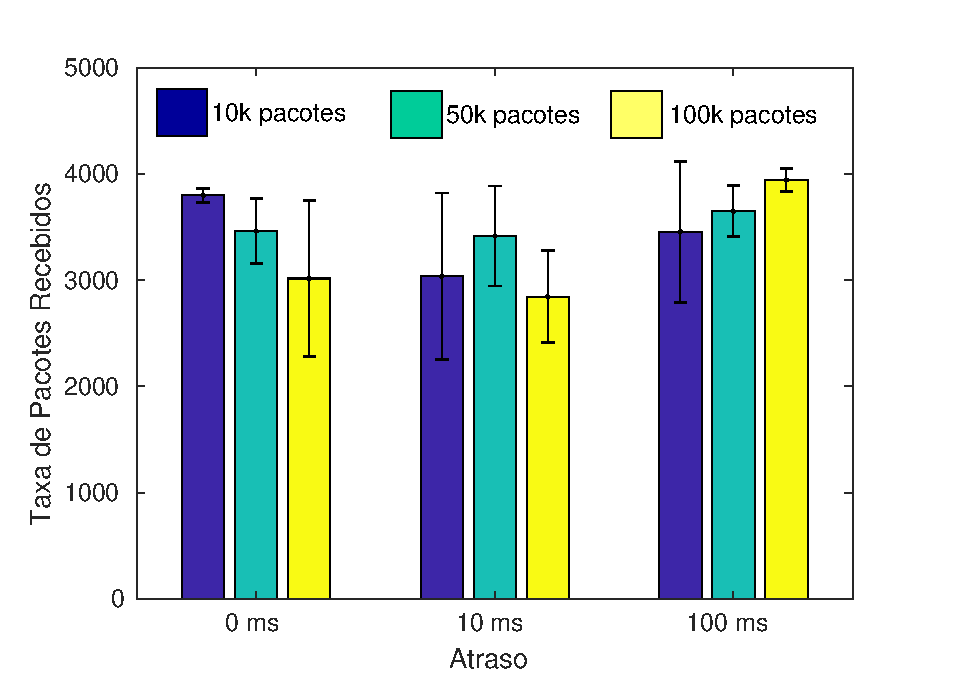
\includegraphics[width=0.45\textwidth]{figs/graficos/taxa64bytes.eps}}
}
%\hspace{-2mm}
% \mbox{
% \subfigure[Pacotes de 400 bytes.] {
% \label{fig:topos:b}
% \includegraphics[width=0.3\textwidth]{figs/graficos/taxa400bytes.eps}}
% }
\hspace{-2mm}
\mbox{
\subfigure[Pacotes de 1200 bytes.] {
\label{fig:taxa:1200}
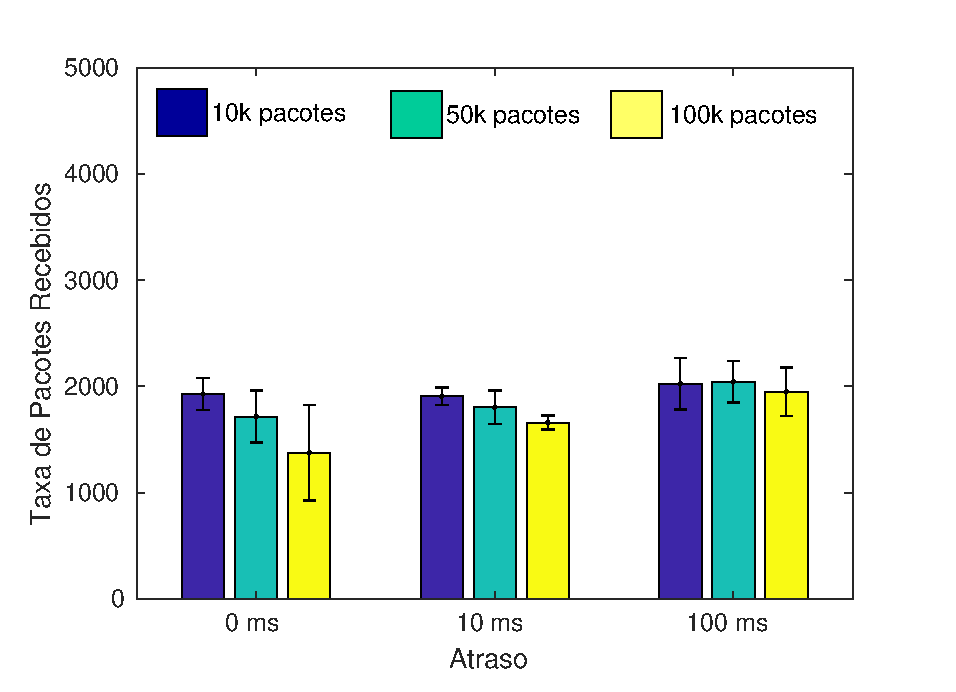
\includegraphics[width=0.45\textwidth]{figs/graficos/taxa1200bytes.eps}}
}
\end{center}
\vspace{-3mm}
\caption{Taxa de pacotes de recebidas pelo consumidor de dados ao realizar envios em taxas superiores à capacidade do enlace sem-fio. O atraso entre o \textit{gateway} e a infraestrutura de virtualização de rede não influencia nas taxas alcançadas. Os experimentos foram realizados com fluxos UDP com pacotes pequenos (a) 64 bytes e pacotes grandes (b) 1200 bytes.}
\label{fig:taxas}
\vspace{-3mm}
\end{figure*}


A segunda etapa da avaliação foca na virtualização da rede sem-fio. A avaliação considera quatro cenários simples de aplicação da infraestrutura de virtualização para IoT. O primeiro cenário contempla o caso em que há um computador conectado a um ponto de acesso virtual 
%%% Pedro: estes labels não estão de acordo com os dos gráficos. Estou mudando para ficar, se achar melhor mudar os labels dos gráficos, lembre de voltar no texto.
%%%Diogo: Vamos deixar os labels do texto iguais aos do gráfico. O gráfico, não consigo mudar daqui do meu notebook. Não tenho o matlab.
(\texttt{1c1ap}); o segundo, 2 computadores em um único ponto de acesso virtual (\texttt{2c1ap}); o terceiro, 1 computador em 2 pontos de acesso virtuais (\texttt{1c2ap}); e, por fim, o último cenário em que há 2 computadores conectados há 2 pontos de acesso virtuais (\texttt{2c2ap}). A Figura~\ref{fig:atraso:wifi} mostra a
%%% Pedro: aqui é a variação do atraso mesmo (Jitter)?
%Diogo: Na verdade é a mudança no atraso quando ocorre a mudança de cenário. Assim, não é o jitter. Para tentar melhorar o entendimento, troquei a preposição para NO atraso em vez de DO atraso.
variação no atraso percebido pelos objetos conectados em cada cenário quando há o acréscimo de latência entre o \textit{gateway} e a NFVI. Nota-se que o atraso percebido pelos nós é mais significativo quando não há latência na conexão do \textit{gateway} (0~ms), já que o tempo de comunicação entre o \textit{gateway} e a NFVI somado à sobrecarga de virtualização da rede sem-fio introduz uma latência da ordem de 10~ms. 
%%% Pedro: aqui não teria que ter uma medida do atraso sem virtualização para você dizer o quanto foi introduzido por ela?
%Diogo: O cenário sem virtualização é o *c1ap
Conforme ocorre o aumento do atraso entre \textit{gateway} e NFVI, 
%%% Pedro: não gostei muito desta frase abaixo:
%o atraso inicial é estatisticamente amortecido pela variação do atraso adicionado. 
%%% Pedro: sugestão de mudança:
o atraso introduzido pela virtualização torna-se menos significativo.
%Diogo: Perfeito! troquei.
O segundo experimento dessa etapa verifica a banda agregada alcançada pelos objetos em cada cenário, Figura~\ref{fig:banda:wifi}. 
%%% Pedro: não entendi esta frase. De onde tirou isso? (abaixo)
%%Diogo: Medi a banda entre um note e o gateway sem nada além do básico para ter a comunicação e verifiquei que a placa só chegava a 18Mb/s.
A banda agregada não é afetada pela virtualização da rede sem-fio para pacotes de 1200~B. A banda agregada aumenta no cenário com dois pontos de acesso e dois computadores. Tal comportamento deve-se ao fato de que ao realizar a virtualização, o escalonamento entre os nós sem-fio é realizado pelo núcleo do sistema operacional do \textit{gateway} em detrimento da realização do escalonamento pelo controlador da placa de rede sem-fio que apresenta um controlador com baixo poder de processamento. 
%%% Pedro: este não seria um resultado interessante para ressaltar, antes e/ou depois?
%%%Diogo: não entendi o que você quer dizer.

%%%%%%%%%%%%%%%%%%%%%%%%%%%%%%%%%%%%%%%%%%%%%%%%%%%
\begin{figure*}[tb!]
\begin{center}
\hspace{-3mm}
\mbox{
\subfigure[Atraso com virtualização do sem-fio.]{
\label{fig:atraso:wifi}
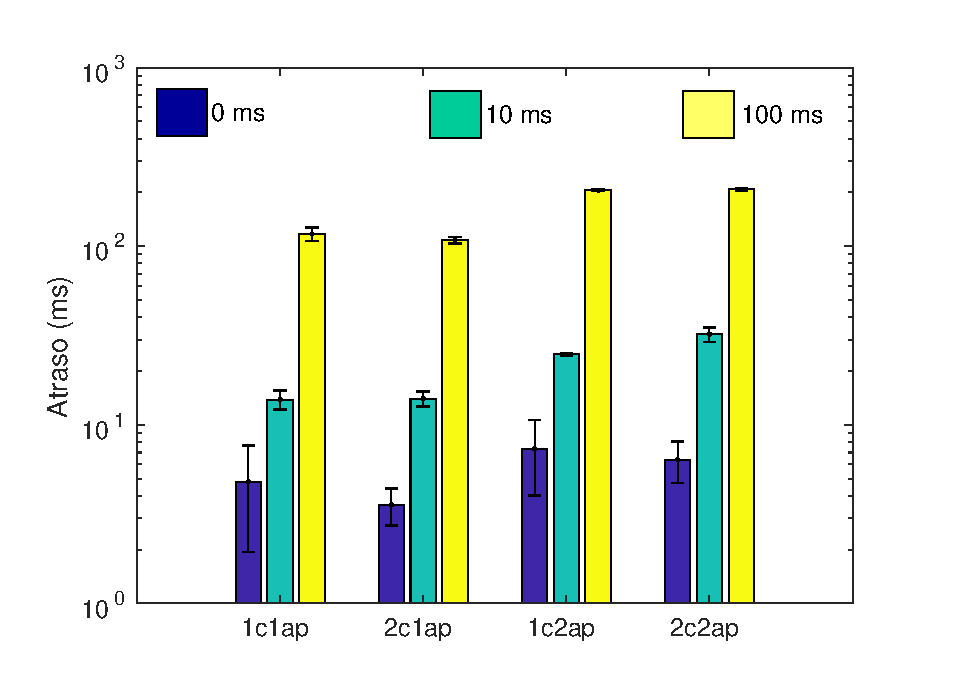
\includegraphics[width=0.45\textwidth]{figs/graficos/atraso-virt-wifi.eps}}
}
% \mbox{
% \subfigure[Pacotes de 400 bytes.] {
% \label{fig:topos:b}
% \includegraphics[width=0.3\textwidth]{figs/graficos/taxa400bytes.eps}}
% }
\hspace{-3mm}
\mbox{
\subfigure[Banda com virtualização do sem-fio.] {
\label{fig:banda:wifi}
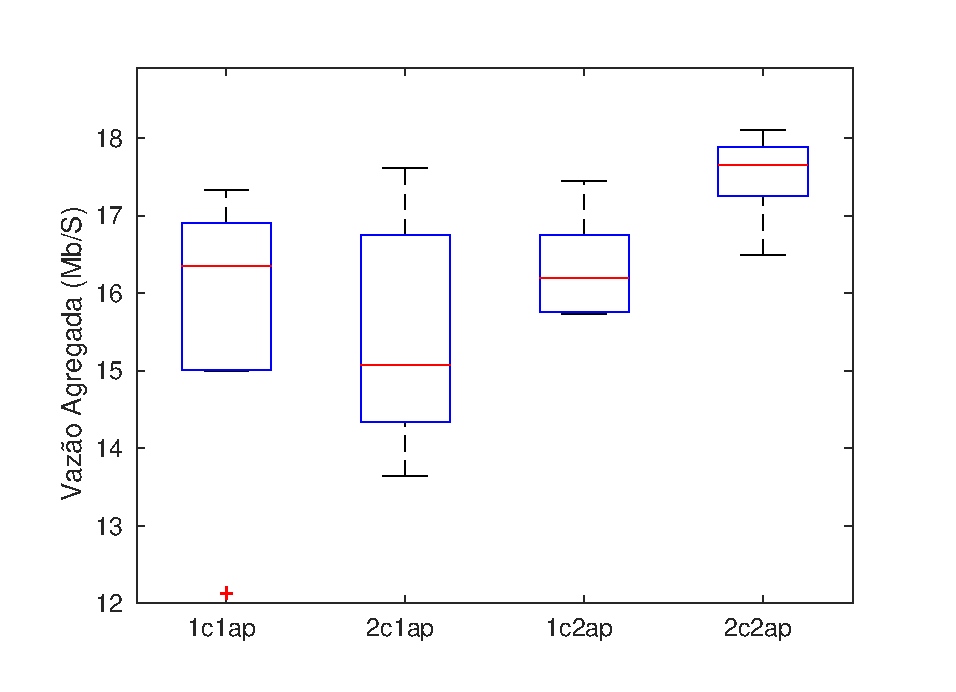
\includegraphics[width=0.45\textwidth]{figs/graficos/vazao-boxplot.eps}}
}
\end{center}
\vspace{-3mm}
\caption{Virtualização do enlace sem-fio. Avaliação dos cenários com 1 computador e 1 ponto de acesso virtual (\texttt{1c1ap}); 2 computadores e 1 ponto de acesso virtual (\texttt{2c1ap}); 1 computador e 2 pontos de acesso virtuais (\texttt{1c2ap}); e 2 computadores e 2 pontos de acesso virtuais (\texttt{2c2ap}). a) O acrescimo no atraso percebido pelos dispositivos conectados é inferior a 10~ms, mesmo quando o atraso entre o \textit{gateway} e a NFVI é de 100~ms. (b) A banda agregada ao usar 2 computadores e 2 pontos de acesso virtuais é, na média, superior aos demais casos.}
\vspace{-5mm}
\end{figure*}

Na terceira e na quarta etapas da avaliação da proposta, considera-se um caso de uso da infraestrutura de virtualização para IoT em que a rede de objetos conectados é compartilhada entre usuários de rede sem-fio, por exemplo celulares inteligentes, e objetos com acesso à Internet, como uma câmera IP. Nesse caso de uso, todos os objetos conectados são susceptíveis a ataques e à infecção por \textit{malware}. Assim, uma possível proteção da rede é instanciação de uma função de rede capaz de classificar o tráfego em legítimo ou tráfego malicioso e posterior adequação do tráfego a políticas. 

A classificação do tráfego entre legítimo e malicioso depende do treinamento e da avaliação de algoritmos de classificação baseados em aprendizado de máquina. Para tanto, foi criado um conjunto de dados de treinamento e teste composto de dados legítimos e dados de ataques rotulados\footnote{O conjunto de dados pode ser obtido através de contato com os autores.}. Os dados legítimos foram coletados durante o uso quotidiano de câmeras IP e de usuários de rede sem-fio no Grupo de Teleinformática e Automação (GTA/UFRJ). Em especial, as câmeras foram acessadas para gerar fluxos de vídeo contínuo, acesso a servidores FTP para transferência de vídeos e fotos e sincronização de data pelo {\it Network Time Protocol} (NTP). Os dados de ataque foram obtidos dos traços coletados por Garcia {\it et al.} em um estudo sobre o comportamento de \textit{botnets}~\cite{botnet}. O conjunto de dados é composto por fluxos identificados pela tupla de endereço IP de origem e de destino, portas de origem e destino e protocolo de transporte~\cite{csnet-martin}. 
%%% Pedro: não captei esta frase abaixo.
%%% Essa é uma frase de "proteção" contra a crítica de usar características de Tag como numéricas. Assim, digo que só usei as numéricas.
As características usadas para geração do conjunto de dados são o subconjunto das características numéricas fornecidas pela aplicação de análise de traços de rede \texttt{flowtbag}\footnote{https://github.com/DanielArndt/flowtbag}, acrescidas de marcações para os 10 serviços mais acessados, em número de fluxos. Esses serviços representam 1\% de todos os serviços acessados no conjunto de dados.

%%%%%%%%%%%%%%%%%%%%%%%%%%%%%%%%%%%%%%%%%%%%%%%%%%%
\begin{figure*}[tb!]
\begin{center}
\hspace{-3mm}
\mbox{
\subfigure[Acurácia da classificação.]{
\label{fig:acc}
\includegraphics[width=0.45\textwidth]{figs/graficos/acuracia.eps}}
}
% \mbox{
% \subfigure[Pacotes de 400 bytes.] {
% \label{fig:topos:b}
% \includegraphics[width=0.3\textwidth]{figs/graficos/taxa400bytes.eps}}
% }
\hspace{-3mm}
\mbox{
\subfigure[Curva ROC para a classe de ataque.] {
\label{fig:roc:pca}
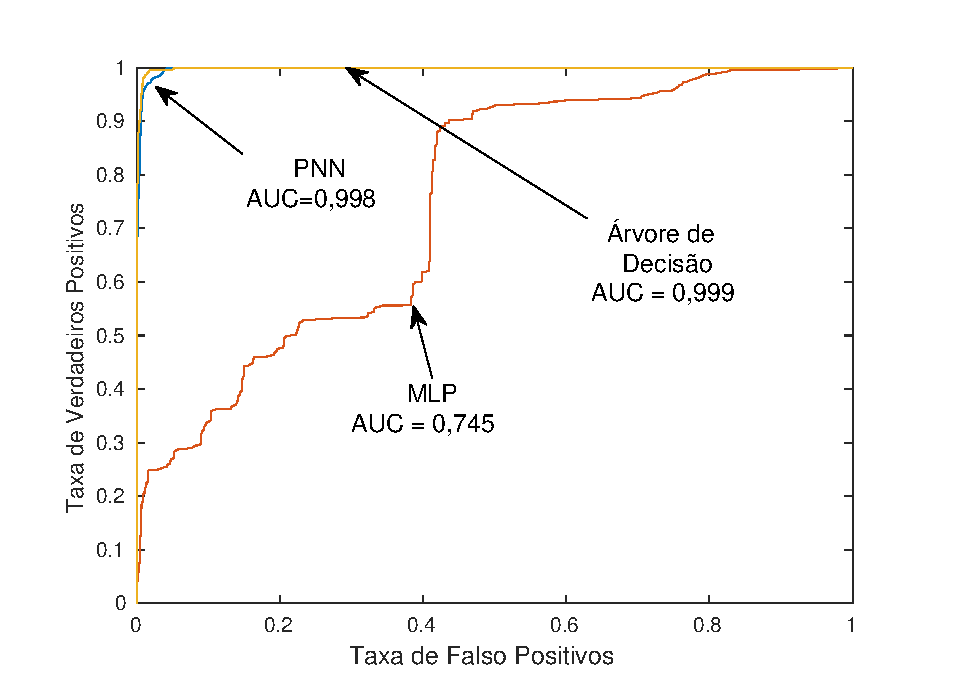
\includegraphics[width=0.45\textwidth]{figs/graficos/roc-pca.eps}}
}
\end{center}
\vspace{-3mm}
\caption{Avaliação de algoritmos de aprendizado de máquina para a classificação de tráfego IoT quando usando PCA para redução de dimensionalidade e usando todas as características. a) A acurácia do classificador baseado em Árvores de Decisão é superior à Rede Neural Probabilística e à Rede Neural com Múltiplas Camadas. b) Comparação das taxas de falsos positivos e verdadeiros positivos dos classificadores. %O algoritmo de Árvores de Decisão é o que apresenta a melhor relação entre verdadeiros positivos e falsos positivos.
\vspace{-3mm}
}
\end{figure*}

%Classificação
\begin{table}[h!]
\vspace{-3mm}
\centering
\caption{Classificação com Árvores de Decisão e redução de dimensionalidade.}
\label{tab:nn}
\begin{tabular}{|c|c|c|c|c|c|c|c|}
\hline
& \textbf{VP} & \textbf{FP} & \textbf{VN} & \textbf{FN} & \textbf{Precisão} & \textbf{Sens.} & \textbf{Espec.}\\ \hline
\textbf{Malicioso}& 14.208 & 290 & 3.995 & 0,00 & 0,98 & 1,00 & 0,93  \\ \hline
\textbf{Normal}& 3.995 & 0 & 14.208 & 290 & 1,00 & 0,93 & 1,00 \\ \hline
\end{tabular}
\end{table}

A Figura~\ref{fig:acc} compara a acurácia de três algoritmos de classificação: rede neural probabilística (\texttt{PNN}); rede neural com múltiplas camadas (\texttt{MLP}) e árvores de decisão (\texttt{Árvores de Decisão}). Os algoritmos foram executados para todas as características e para o cenário em que a dimensionalidade do problema foi reduzida usando-se a análise de componentes principais (PCA). Nota-se que a classificação usando árvores de decisão treinadas com o algoritmo de {\it gradient boosting} apresenta a melhor acurácia quando comparada com redes neurais. Tal comportamento é esperado dada a natureza discreta dos dados dos fluxos, em que a segmentação binária dos dados, conforme é feita pelo algoritmo de árvore de decisão, leva a regras de classificação acuradas. Quando compara-se a relação entre taxa de verdadeiros positivos e falsos positivos dos algoritmos de classificação, curva ROC mostrada na Figura~\ref{fig:roc:pca}, as árvores de decisão apresentam uma área abaixo da curva (AUC) muito próxima a 1, indicando que a classificação dos dados não incorre na geração de falsos positivos, nem falsos negativos, para a classe de ataque. A redução da dimensionalidade para apenas 8~componentes principais manteve 99\% da informação do conjunto de dados e tem acurácia praticamente igual à classificação com todas as características.
A Tabela~\ref{tab:nn} mostra o desempenho das árvores de decisão, com dimensionalidade reduzida pelo PCA, em uma avaliação cruzada em $10$ rodadas\footnote{VP: Verdadeiro Positivo; FP: Falso Positivo; VN: Verdadeiro Negativo; FN: Falso Negativo; Sens.: Sensibilidade; Espec: Especificidade.}. A acurácia nominal desse foi de $0,998$, com sensibilidade de $1,0$ no tráfego malicioso.
%%% Pedro: não precisa definir a fórmula da precisão?
%%Essa é uma medida "padrão". Se eu for defini-la, teria que fazer o mesmo para todas as outras que apresento.

Por fim, na quarta etapa, avalia-se a capacidade de a infraestrutura de virtualização proposta tomar contramedidas e aplicar políticas aos pacotes. A Figura~\ref{fig:diff-serv} mostra o resultado do experimento em que dois computadores portáteis conectados à rede sem-fio têm acesso a qualidade de serviço (QoS) distintas. A diferenciação do serviço é provida por uma VNF através do direcionamento do tráfego dos nós para filas distintas. As filas são implementadas em um comutador por \textit{software} Open vSwitch. No experimento, ambos os nós executam um fluxo TCP na vazão máxima que alcançam. Um dos nós é direcionado a uma fila com garantia mínima de recurso de banda a 5~Mb/s. O outro nó tem uma garantia mínima de 1 Mb/s. A Figura~\ref{fig:diff-serv} ressalta que após 30~s, os limites das filas são configurados e os fluxos passam a ser conformados pelos limites, garantindo ao tráfego de maior recurso reservado banda total, útil mais encapsulamento, próxima aos 5~Mb/s, em detrimento do outro nó que não possui recursos dedicados. 


%%%%%%%%%%%%%%%%%%%%%%%%%%%%%%%%%%%%%%%%%%%%%%%%%%%
\begin{figure*}[tb!]
\begin{center}
\hspace{-3mm}
\mbox{
\subfigure[Diferenciação entre fluxos.]{
\label{fig:diff-serv}
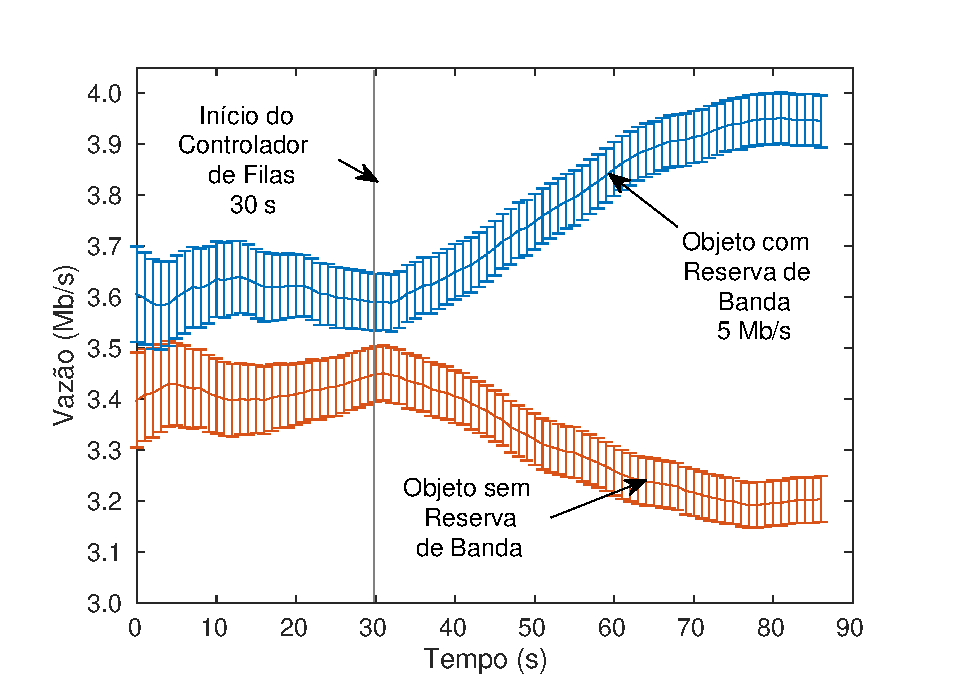
\includegraphics[width=0.45\textwidth]{figs/graficos/diffserv.eps}}
}
% \mbox{
% \subfigure[Pacotes de 400 bytes.] {
% \label{fig:topos:b}
% \includegraphics[width=0.3\textwidth]{figs/graficos/taxa400bytes.eps}}
% }
\hspace{-3mm}
\mbox{
\subfigure[Ataque de negação de serviço na rede.] {
\label{fig:dos}
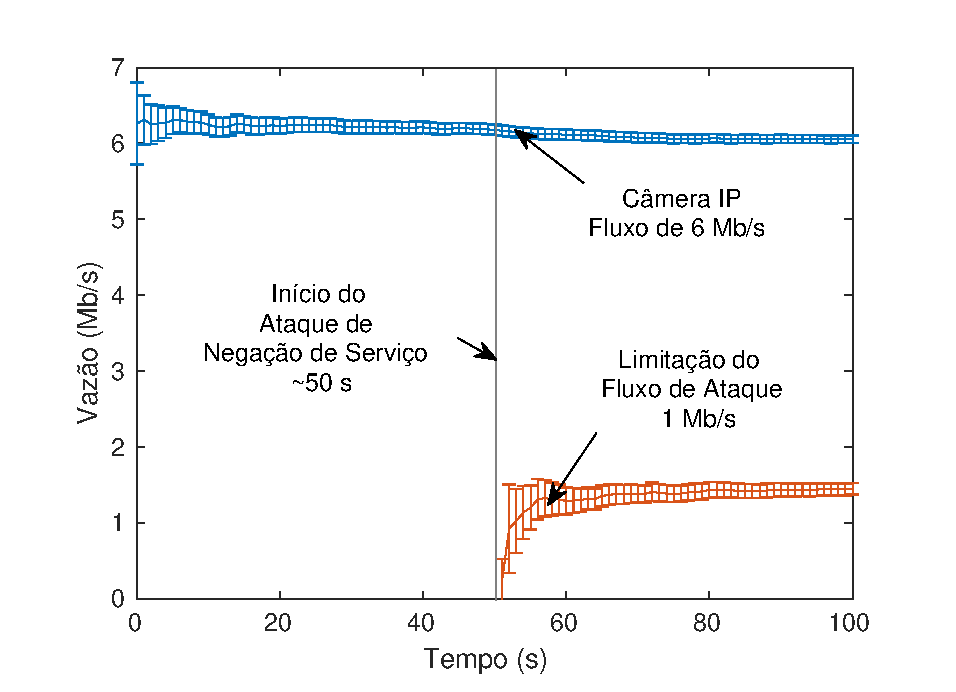
\includegraphics[width=0.45\textwidth]{figs/graficos/dos.eps}}
}
\end{center}
\vspace{-3mm}
\caption{Diferenciação entre fluxos no cenário de IoT. a) Dois objetos conectados compartilham a rede sem-fio e enviam tráfego UDP constante a 5~Mb/s. Em 30~s, o controlador de recursos de banda é ativado. Um objeto tem 5~Mb/s garantido por política e o outro só tem um mínimo garantido de 1~Mb/s. b) Cenário de ataque de negação de serviço na rede de sensores com uma câmera IP e um nó. O fluxo classificado como legítimo da câmera IP tem mínimo de 6~Mb/s garantidos pela política de filas. O fluxo não-legítimo é limitado a 1~Mb/s.}
\vspace{-3mm}
\end{figure*}

A Figura~\ref{fig:dos} mostra o cenário em que uma câmera IP está enviando um fluxo de vídeo contínuo TCP de aproximadamente 6~Mb/s quando ocorre um ataque de negação de serviço (DoS). O ataque de negação de serviço é configurado como um fluxo UDP de 20~Mb/s. No entanto, mesmo a câmera tendo uma configuração de \textit{hardware} inferior ao computador portátil atacante, a função de rede virtualizada consegue garantir a taxa de transmissão estável para a câmera, enquanto limita o tráfego classificado como malicioso a aproximadamente 1~Mb/s, evitando assim a degradação do serviço provido pela câmera.

\section{Trabalhos Relacionados}
\label{sec:relacionados}

Petrolo {\it et al.} argumentam que cidades inteligentes é uma aplicação de Internet das Coisas no domínio das cidades e destacam os benefícios da integração de diversos dispositivos conectados. Os autores definem o conceito de Nuvem de Coisas ({\it Cloud of Things} – CoT) que consiste no uso de ambientes de computação em nuvem para prover uma plataforma de integração de silos de dados de IoT~\cite{petrolo}. Santana {\it et al.} ratificam a ideia de cidades inteligentes composta por objetos conectados e argumentam que a quantidade de dados gerados em cidades inteligentes é grande e requer uso de técnicas próprias para {\it Big Data}~\cite{interscity-paper}. Assim, Santana {\it et al.} vislumbram a arquitetura de cidades inteligentes como uma agregação de processamento em nuvem com sistemas ciber-físicos ({\it Cyber-Physical Systems} – CPS).

%Zhang \textit{et al.}  identificam diversas aplicações que executam sobre as plataformas de cidades inteligentes, tais como, energia inteligente, ambiente inteligente, indústria inteligente, casas inteligentes e serviços públicos inteligentes. Os autores argumentam que é necessário prover uma arquitetura de gestão e processamento de dados consciente dos requisitos de segurança e de privacidade dos dados~\cite{zhang-security}.

Atzori {\it et al.} comparam as características de sistemas de identificação por rádio frequência (RFID)
%%% Pedro: a frase acima, está correta? É isso mesmo: RFID duas vezes?
%%% Diogo: Era assim que estava no paper.
, redes de sensores sem fios e redes de RFID.  Os autores evidenciam que os sistemas RFID são pequenos, de baixo custo e energia não é limitante. As redes de sensores sem fio apresentam alta cobertura de rádio e a comunicação não requer a presença de um leitor,
%%% Pedro: não entendi esta frase abaixo:
%%%Diogo: Mudei um pouco para ficar mais claro.
enquanto nos sistemas RFID, leitor e sensor são assimétricos.
As redes de sensores RFID possibilitam a detecção, computação e comunicação em um sistema passivo~\cite{survey-morabrito}. Por sua vez, Adelantado {\it et al.} investigam as limitações do padrão LoRaWAN~\cite{lorawan}. Assim, cada rede de acesso diferente para os dispositivos de IoT apresenta características e requisitos de redes distintos. 

Quin \textit{et al.} propõem 
%uma arquitetura de
um {\it middleware} baseado em 
redes definidas por {\it software} para Internet das Coisas. A ideia consiste em prover múltiplos ambientes de rede para IoT para atender demandas de rede com diferentes requisitos~\cite{sdn-iot}. 
%Quin \textit{et al.}, então, propõem um {\it middleware} capaz de monitorar a rede e adaptá-la de acordo com as necessidades das tarefas executadas~\cite{sdn-iot}. 
Para tanto, a proposta monitora a rede e usa cálculo de rede para prever a mudança no desempenho. A proposta Black SDN, por sua vez, propõe o uso de redes definidas por {\it software} para prover segurança em redes de IoT através da criptografia tanto do conteúdo quanto dos cabeçalhos dos pacotes~\cite{black-sdn}. %Para tanto, o roteamento dos pacotes na rede é realizado pelo controlador da rede que é a âncora de confiança e, portanto, detém a chave para decifrar os pacotes e instalar regras na rede de acordo com o roteamento correto.

Bizanis e Kuipers investigam o emprego de virtualização e redes definidas por {\it software} em ambientes de Internet das Coisas~\cite{sdn-nfv-iot}. Os autores concluem que a virtualização de rede e as redes definidas por {\it software} são facilitadores da Internet das Coisas, mas focam somente no uso dessas tecnologias como forma de gerenciar os fluxos gerados por objetos conectados. 
Ojo {\it et al.} defendem que arquiteturas e protocolos de rede tradicionais são ineficientes para suportar o alto nível de escalabilidade, a grande quantidade de tráfego e a mobilidade dos dispositivos de IoT. Além disso, é difícil gerenciar a quantidade de dados gerada, o que pode causar problemas e interrupções na rede~\cite{globecomm-nfv-iot}. Assim, os autores propõem que a rede de transporte de dados de IoT seja gerenciada com aplicações sobre as redes definidas por {\it software} e com funções de rede implementadas em funções virtuais de rede. Contudo, os autores não focam na criação de domínios de IoT isolados que compreendam desde o acesso até o consumo.
%%% Pedro: não entendi esta última parte da frase acima.
%%% Diogo: Para dizer que eles não propõem a virtualização que a gente faz! ;-)

%, nem definem como deve ser a gerência e o desenvolvimento dessas funções.

A infraestrutura de rede de transporte proposta nesse artigo baseia-se em um {\it gateway} simples que encaminha todos os pacotes dos objetos conectados para um ambiente de virtualização de funções de rede. Diferentemente das propostas anteriores, esse trabalho foca na rede de transporte dos dados, independentemente, do {\it middleware} ou da plataforma de IoT utilizados. As funções exercidas pela rede de transporte compreendem o encaminhamento de pacotes, a adequação a políticas e a adaptação de dados.%, entre outras. %Ademais, outro diferencial do trabalho é reação a anomalias da rede em tempo real através da execução de mecanismos de inteligência de máquina


\section{Conclusão} %(0,5 página)
\label{sec:conclusao}

O número de objetos conectados é cada vez maior e a criticidade dos dados trafegados também. Contudo, as redes de transporte de dados para Internet das Coisas é preterida em relação à aquisição e ao processamento dos dados. Esse artigo propôs uma infraestrutura de virtualização de funções de rede que permite a implantação ágil e efetiva de funções virtuais. A proposta desenvolveu a ideia de um nó de acesso virtualizado capaz de criar domínios independentes de objetos conectados. Em cada domínio são aplicadas funções de rede independentes e ajustadas para os requisitos de desempenho e segurança de cada aplicação de Internet das Coisas. Um protótipo da infraestrutura proposta foi desenvolvido e avaliado. Os resultados demonstram que o nó de acesso virtualizado não introduz perda de desempenho para o acesso dos objetos conectados. Verificou-se ainda que a latência entre o nó de acesso e a infraestrutura pode ser substancialmente alta sem que haja perdas de desempenho. Por fim, foi desenvolvido um caso de uso da infraestrutura proposta, em que uma função virtual de rede foi capaz de classificar o tráfego entre legítimo ou malicioso com 99,8\% de acurácia e, em seguida, uma outra função virtual garantiu qualidade de serviço ao tráfego legítimo e limitou um ataque de negação de serviço impedindo que o serviço essencial de uma câmera IP fosse degradado. 

%Como trabalhos futuros, pretende-se desenvolver novas funções de rede virtuais, como funções de adaptação de protocolo de aplicação e sistemas de detecção de intrusão baseados em inspeção profunda de pacotes para Internet das Coisas.

%referenicas
%%Padrão
% \bibliographystyle{apalike_br}
% \bibliography{biblio}

% %%%Condensado
\begin{spacing}{0.85}
%\begin{footnotesize}
\begin{normalsize}

\bibliographystyle{apalike_br}
\bibliography{biblio}

\end{normalsize}
\end{spacing}

\end{document}
